\chapter{用户转发行为分析}
\label{ch6}

\section{引言}
\label{ch6_intro}
上一章介绍了如何从社交媒体用户产生内容中挖掘出话题和观点信息并在用户层面集成对用户的主观性进行建模,本章主要介绍如何应用主观模型对用户在信息传播中的转发行为进行分析。

信息传播通过逐步层叠式的信息扩散触发大量用户参与到信息的病毒式传播中,在市场营销、政治选举等应用场景中发挥着重要作用,引起了众多研究者,尤其是社交网络研究人员的广泛关注。社交网络研究为信息传播设计了一些通用的传播模型,可以进行模拟信息流动(Information flow)\upcite{Goldenberg2001,Kempe2003}以及探测信息瀑布(Information cascades)爆发\upcite{Cheng2014}。但是这些模型都是将用户看作是网络中的一个简单节点,忽视了用户在信息传播过程中的行为自主性。作为社交媒体中的信息消费者和产生者,每个用户都可以在社交媒体上发帖和转贴以表达自己的兴趣和观点,能自主选择信息和传播信息。在社交媒体中一条信息能否得到广泛传播主要依赖于用户间的“口碑(Word of mouth)”效应,只有口碑效应好的信息才会引起广泛用户的兴趣对其进行传播,口碑效应取决于用户信息消费的主观意图,因此分析用户的主观意图可以对促进信息的传播研究。随着自然语言处理(Natural Language Processing)和数据挖掘(Data mining)技术的发展,社交媒体用户的主观意图可以使用用户自己产生的数据进行建模来分析。本章就是基于口碑效应机制问题,研究给定某个用户的一条微博,分析所有收到该微博用户中谁最有可能参与到该条微博的后续传播中。一个典型的场景是,在如图~\ref{fig6-0}所示Twitter的一个异构网络中,用户Tony和关注他的所有朋友在以往的信息交流中讨论了两个话题:“苹果手机(Iphone)”以及电影“冰雪奇缘(Frozen)”,要研究的问题是:Tony新发布了一条有关电影“冰雪奇缘”微博,如何判定他所有朋友中谁会转发传播这条微博?

\begin{figure}[htb]
\centering
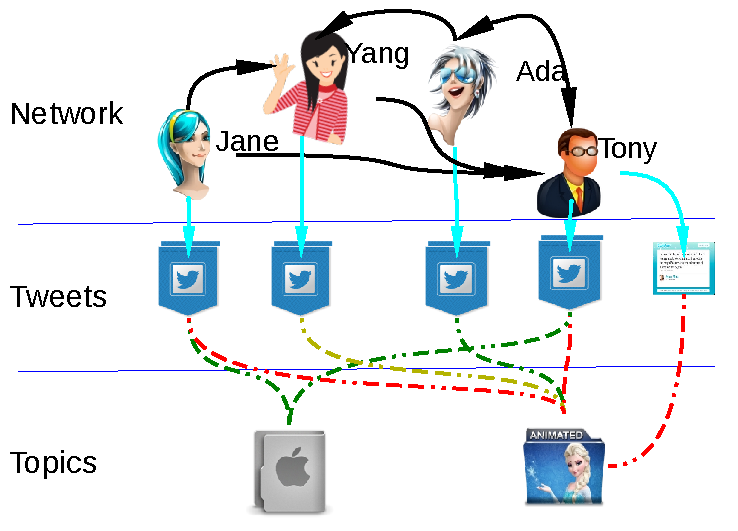
\includegraphics[height=180pt]{6-0.pdf}
\caption{问题示意图}
\label{fig6-0}
\end{figure}
%\footnotetext{每个用户的观点用不同颜色表示,“红色”当标正面观点,“绿色”代表负面观点,“黄色”代表中性观点。}

不同社交网络平台上的信息传播行为是不一样的,本章主要分析Twitter用户的微博转发行为。庞大的用户群以及信息的指数级增长,使得Twitter在互联网的信息传播中扮演着重要角色。尽管Twitter微博在长度上受到限制,但是Twitter提供用户间转发机制为信息的快速传播提供了前所未有的便捷途径。据有关统计,Twitter中有超过四分之一的微博是由用户间的相互转发形成的\upcite{yang2010understanding},因此理解了用户的转发行为就能够很好的解释Twitter上的信息传播。

社交媒体用户是信息传播的参与者,同时也是个性化的信息消费和生产主体,用户很自然地会在信息的交互中表达出自己兴趣和观点,表现出主观性。在心理学的研究中证实了人的主观能动性(Subjective initiative)决定了人的主观性会影响自己的行为模式\upcite{Moore2008},同样根据偏颇吸收(Biased Assimilation)理论,人总是趋向于选择跟自己偏执化观点(Biased opinions)相一致的信息进行传播\upcite{Hyman2000}。因此用户的主观性是研究用户参与信息传播意图的一个很重要的方面。转发行为分析研究提出了一些方法和模型来确定一些影响转发行为的因素\upcite{Macskassy2011,Feng2013}。但是目前还没与相关工作关注到用户转发行为的主观动机。从Twitter的口碑效应来看,转发行为是一个连续的过程,包含着接收到微博,对微博内容评估,最后确定时候转发三个环节。三个环节中最重要的就是评估微博内容是否有价值的信息值得和朋友分享,也就是用户转发行为的主观动机。因此对用户的主观动机进行建模会为转发行为分析提供重要的研究视角。依据“物以类聚(Like attracts like)”原则,用户更容易转发那些能够迎合他个人口味的信息。以图~\ref{fig6-0}中的例子来说明,每个用户对网络中谈论的两个话题所持观点可以从他们历史发布的微博中得出,假设Tony和Jane对电影“冰雪奇缘”持正面肯定观点,而Ada持负面观点,Yang持中性观点。如果Tony新发布的微博内容是对冰雪奇缘表达正面肯定的观点,应该可以确定Jane是最有可能转发这条微博的用户。从这种动机出发,本章主要研究用户的主观性是如何影响其转发行为。

为了研究主观性和转发行为的关系,需要回答两个问题:(1)怎样准确对用户的主观性进行建模?(2)怎么样从用户的主观性角度度量微博值得传播?
上一章内容已经提出了使用观点集成方法来对社交媒体上用户主观性建模,并定义了社交媒体用户的主观模型及其构建方法。本章将继续使用主观模型概念,并针对用户的转发行为分析提出一个新的主观相似性计算方法来度量微博是否值得传播,针对影响转发行为的三个因素,即微博内容的吸引力、转发行为的社交需求以及从众需求(Conformity needs)\upcite{Cialdini2004},定义三个主观相似性度量三个因素对转发行为的影响。

\section{相关工作}
\label{ch6_relatedwork}
在微博转发行为分析方面,已经有大量工作在转发行为特征分析、提高微博转发性因素确定以及设计模型估计转发概率三个方面展开研究。例如Suh等~\upcite{suh2010want}发现带有Url网络连接以及hashtag标记的微博更有可能被转发;Macskassy和Michelson~\upcite{Macskassy2011}发现从微博内容中推理得到的模型能够解释大多数的转发行为;Comarela等\upcite{comarela2012understanding}发现与微博作者前期交互,微博作者发帖频率,微博内容的新鲜程度以及微博的长度会影响关注者的转发行为;Starbird和Palen~\upcite{starbird2012will}特别针对危机发生时的微博信息转发机制进行了研究,发现有危机话题关键词的微博更有可能被转发;Osborne和Lavrenko~\upcite{petrovic2011rt}通过引入一些特征,比如微博的新颖性和作者被加入朋友列表的次数,使用被动攻击算法(Passive aggressive algorithm)训练模型预测转发行为;Jenders等~\upcite{jenders2013analyzing}从微博及其作者的网络结构、信息内容以及情感信息分析了一些“显式”和“隐式”的影响转发的特征;Naveed等~\upcite{NaveedGKC2011,naveed2011searching}
引入了微博的趣味性指标,并使用表情符、情感以及话题等特征对趣味性指标进行量化来预测微博被转发的可能性;Feng和Wang~\upcite{feng2013retweet}构建了一个图模型,并将微博以及用户的所有信息组合到图的节点和边的信息里面,并提出了一个因子分解模型(Factorization model)对微博依据被转发的概率进行排序;Pfitzner等~\upcite{Pfitzner2012}提出了一种叫做情感分歧(emotional divergence)指标来评价微博被转发的可能性,并研究证实了高情感分歧值的微博会有更高的机会被转发;Luo等\upcite{Luo2013}设计了包括转发历史特征、用户特征、用户活跃时间特征以及用户兴趣特征四组特征集合对用户转发微博行为进行分析,并根据转发可能性对用户排序。

总体来说,上述所有工作主要是回答“哪些微博会否被什么样的用户转发”这样一个问题,但是忽略了用户在转发时的主观动机,也就是“站在用户角度,某条微博是否值得用户转发”这样的问题,本章将结合上一章提出的主观模型从用户用户的主观动机角度来分析转发行为。

\section{基于主观模型的转发分析}
为了研究用户转发行为的主观动机,首先需要了解用户的主观性,也就是弄清楚用户喜欢什么和不喜欢什么(即用户感兴趣的话题和用户对话题所持的观点),这就是上一章为用户所建立主观模型的用途,通过用户主观模型可以清楚了解用户的主观性,为分析用户的转发行为分析提供信息基础。从技术角度来讲,上一章提出的主观模型的目标就是设计一个通用的框架能够从社交媒体用户产生历史数据中同时获得用户兴趣(对应的话题分布)和全面的观点(对应的观点分布)信息,为后续的一些应用提供信息支持。之所以主观模型是通用的,因为它不但将用户的兴趣和观点结合进一个整体框架,更重要的是,在主观模型中观点表示为一个在可扩展的情感表示空间上的概率分布。这个情感表示空间既可以是表示情感正负极性的二值空间,又可以是连续值表示的情感强度空间,或是离散值表示的情绪类型空间,因此可以覆盖所有的观点表示形式。这种观点的表示形式一方面可以在细粒度的情感值空间区别不同观点,另外一方面可以以概率分布计算不同观点之间的相似性,能够准确区分观点和判断观点相似性是对用户主观动机分析的基础。本节主要定义主观相似性为转发行为的主观动机分析提供有效的度量手段。


%随着社交媒体普及率越来越高,社交媒体上带有用户主观性信息的用户产生内容(UGC)也越来越多,自然语言处理领域的观点挖掘(opinion mining)\upcite{Liu2012}研究开始通过计算方式自动对用户的观点信息进行建模。并且也出现了一些基于方面(aspect-based)情感分析或话题情感模型(topic-sentiment model)\upcite{Lek2013,Mei2007}将针对话题的观点投射为二值极性,评价等级或情绪类型等某一个单一的情感值,但是这些模型因为这种观点简单的表示形式而使得其作用受到限制。因此在主观模型中,我们通过将话题和观点结合为一个模型并将话题和观点使用新的表示形式(在话题空间和情感空间的分布)来对用户的主观性进行建模。

\subsection{主观相似性}
\label{similarity}
%Twitter用户一般会对感兴趣的多个不同话题发表观点和看法,比如图~\ref{fig6-0}中的例子中Tony和Jane都对苹果手机话题和冰雪奇缘电影感兴趣并表达了自己的观点。
%一般来讲,用户对话题的兴趣度会随着话题的不同而不同,而且,即便对同一个感兴趣话题,当一个用户其其不同的方面(aspects)发表微博表达的观点也不是完全一样的,因此我们认为对用户的主观性进行建模时:
%\begin{itemize}
%\item 每一个用户$ u $都对应着一个在话题空间$ T $的$ |T| $维的话题分布$ W_{u}=\{w_u(t)\}|W_u \in R^{|T|},\sum_{t}w_{u}(t)=1 $,其中$ w_{u}(t) $表示用户在话题$ t $上的兴趣度。
%\item 用户$ u $对话题$ t $的观点应该表示为一个在情感空间$ S $的$ |S| $维的情感分布$ O_t=\{d_{u,t}(s)| O_t \in R^{|S|}, \sum_{s}d_{u,t}(s)=1\}$,其中$ d_{u,t}(s) $表示用户观点中带有情感值$ s $的可能性。
%\end{itemize}


%图~\ref{fig6-1}是一个在$ [0,100] $话题空间和$ [0,8] $情感强度空间主观模型的可视化示例。
%
%\begin{figure}[htp]
%\centering
%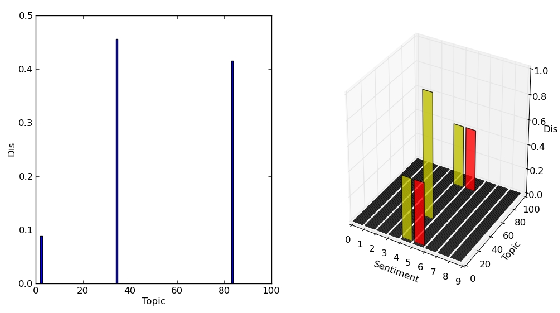
\includegraphics[height=170pt]{6-1.pdf}
%\caption{可视化主观模型示例}
%\label{fig6-1}
%\end{figure}
%左侧图中表示用户在话题2,32和83上的兴趣度:$$ (  w_{u,2}=0.08,w_{u,32}=0.48, w_{u,83}=0.44)  $$
%右侧图中表示在每个话题上的观点分布:
%$$ O_{2}=( d_{u,2,4} =0.5, d_{u,2,5} =0.5)$$
%$$O_{32}=(d_{u,32,4}=1.0) $$ $$O_{83}=( d_{u,83,4}=0.5, d_{u,83,5}=0.5 )$$

构建主观模型框架是将话题分析和观点分析分开进行的。具体来讲,首先使用用户层面(user-level)的LDA话题模型从用户所有的微博$M_u$中训练一个全局话题模型$ TM=(\theta,\beta) $,其中$ \theta $表示用户在话题空间$ T $的兴趣度分布,$ \beta $表示话题在词表上的分布。由于微博比较短小,通常认为每条微博谈论的是一个话题,因此可以通过计算微博$ t $从话题模型中产生的概率值,为$ t $指定一个最有可能的话题:
\begin{equation}
\label{eq6-1}
z_{t} = \arg \max_{k}\prod_{w \in t} P(w|\phi_{k})
\end{equation}

然后就可以将用户$ u $所有谈论同一话题的微博数目进行归一化后获得用户在话题上的兴趣度:
\begin{equation}
w_{u,k}=\dfrac{|\{ t: t \in M_{u} \wedge z_{t}=k\}|}{|M_{u}|}
\end{equation}

至于观点的分布式表示,正如在图~\ref{fig6-0}中的例子,虽然Tony和Jane总体上都是对电影“冰雪奇缘”持正面观点,但是他们有可能是因为不同的原因而喜欢这部电影的。Jane可能非常喜欢电影浪漫的故事情节,但是对它的动画画面稍微有点失望;而Tony喜欢这部电影可能是因为被这部电影的动画技术所折服,却不喜欢它略显幼稚的公主王子题材。情感分析研究主要是将观点表示为单一值,尤其是正负极性二值为主,并不区分针对话题的观点在不同方面的具体观点,也无法计算观点的大小顺序,比如那个用户更喜欢电影。在主观模型中,观点被定义为在情感表示空间$ S $的概率分布,可以更精确的表示和区分观点。假设微博$ t $通过情感分析得出情感值为$ s_t $,用户在某一话题$ k $上的观点分布可以将所有谈论该话题微博在每一个情感值上的数量归一化后获得:
\begin{eqnarray}
O_k &= & \{ d_{u,k,s}|s \in S \} \nonumber \\
  &=& \{ \dfrac{|t:t \in M_u \wedge z_t=k \wedge s_t=s|}{|M_u|}|s \in S\}
\end{eqnarray}

为了量化“物以类据(like attracts like)”这样的效应,得到用户的主观模型后,需要定义一个相似性度量方法来计算用户之间或用户与微博之间主观上的相似性。首先定义在同一话题上两种观点的相似性计算方法。
 
\subsubsection{观点相似性}
\label{opsim}

在主观模型中观点是定义在情感空间上的分布,分布的每一维都代表着在对应情感值上的观点权重。为了区分观点,可以定义情感表示空间中的情感值不独立,情感值之间按照一定的顺序和大小来表示情感的强度。比如情感值为8的观点比情感值为5的观点持更正面的观点。这种情况下常用的一些计算分布相似性的方法,比余弦相似性(cosine similarity)以及KL距离(KL-divergence),对于主观模型中观点分布相似性的计算就不适合。例如表~\ref{tab6-1}所示的三个观点分布,代表在一个$ S=[0,8 ] $情感表示空间中的三个观点:观点$ O_{k}^{1} $是最负面(100\%分布在情感值0上),观点$ O_{k}^{2} $是正面的(50\%分布在情感值6,50\%分布在情感值7上),观点$ O_{k}^{3} $最正面(100\%分布在情感值8上)。
\begin{table}[htb]
%\scriptsize
\centering
\caption{观点相似性示例}
\label{tab6-1}
\begin{tabular}{|l|l|l|l|l|l|l|l|l|l|}
\hline
 观点& 0 & 1& 2 & 3 & 4 & 5 & 6 & 7 & 8 \\
\hline
$O_{k}^{1}$ & 1.0 & 0.0 & 0.0 & 0.0 & 0.0 & 0.0 & 0.0 & 0.0 & 0.0 \\
\hline
$O_{k}^{2}$ & 0.0 & 0.0 & 0.0 & 0.0 & 0.0 & 0.0 & 0.5 & 0.5 & 0.0 \\
\hline
$O_{k}^{3}$ & 0.0 & 0.0 & 0.0 & 0.0 & 0.0 & 0.0 & 0.0 & 0.0 & 1.0 \\
\hline
\end{tabular}
\end{table} 

使用常规的分布相似性计算方法(余弦相似性或KL距离),就会发现三个观点之间的相似性都是0,因而出现了相似性计算方法失效现象,这是与实际不相符的,因为观点$ O_{k}^{2} $与观点$ O_{k}^{3} $比观点$ O_{k}^{1} $与观点$ O_{k}^{3} $更相似,它们都是持正面观点。因此观点的相似性计算不能简单将观点视为一般的概率分布来计算,或者只是情感表示空间的一个距离值。为了准确计算观点之间的相似性,需要将观点在情感表示空间的距离和分布上的相似性结合起来,在此提出了如下的计算观点$O_{k}^{u},O_{k}^{v} $之间相似性方法:
\begin{equation}
\label{opinionsim}
Sim(O_{k}^{u},O_{k}^{v})=\dfrac{|S|-|\sum_{i=0}^{|S|}d_{i}^{u}v_{i}-\sum_{i=0}^{|S|}d_{i}^{v}v_{i}|}{|S|}
\end{equation}
其中$ d_{i} $是第$ i^{th} $维的情感值上的分布,$ v_{i} $是相应的情感值。
使用方法~\ref{opinionsim}计算表~\ref{tab6-1}中观点之间相似性为:
$$ Sim(O_{k}^{1},O_{k}^{3})=0 $$ 
$$Sim(O_{k}^{2},O_{k}^{3})=6/8$$
$$ Sim(O_{k}^{1},O_{k}^{2})=2/8 $$
计算结果达到了与三个观点之间相似性的直觉理解一致的效果。

\subsubsection{主观相似性}
在主观模型中,用户感兴趣的话题表示为在话题空间$ T $上不同话题的兴趣度分布,因此两个主观模型$SM_u$和$SM_v$之间的主观相似性可以将话题上的权重与对应的观点分布相似性结合起来进行集成计算:
\begin{equation}
\label{subsim}
Sim(SM_{u},SM_{v})=\sum_{k=1}^{|T_{u,v}|}\theta_{u}(k)\* Sim(O_{k}^{u},O_{k}^{v})
\end{equation}
其中$ T_{u,v} $表示两个用户之间的共同话题,是两个用户之间感兴趣话题的交集;$ \theta_{u}(k) $代表用户$ u $在话题$ k $上的兴趣度权重。

值得注意的是,当测量用户$ u $在主观性上与用户$ v $有多相似性时,话题权重使用的是用户$ u $的话题权重,因此这个主观相似性度量方法是不对称的。之所以这样设计,是因为考虑到用户的主观上的相似性是个人主观判断,因此度量目标用户与自己主观想法上有多相似是根据个人的话题兴趣度以及观点相似性来确定的,不需要目标用户也作对称性的考量。因此在度量两个用户的主观相似性时,$ Sim(SM_u,SM_v)\neq Sim(SM_v,SM_u)$。

\subsection{转发行为分析}
\label{retweet}
用户的转发行为受到多种因素的影响,从用户的角度来讲,三种情形下会引发用户的转发:
\begin{enumerate}
\item 微博的内容对用户具有吸引力,因此用户的转发行为是根据自己的主观判断引发的;
\item 微博是由关系密切的好朋友发布的,因此用户的转发行为是因为社交需求;
\item 微薄内容是突发新闻或有趣段子,具有流行性,因此用户的转发行为是趋同需求(或称为从众需求,conformity needs)\upcite{Cialdini2004}的结果。
\end{enumerate}
这三种因素是用户产生转发行为的不同原因,从主观动机角度分析,可以使用三个主观相似性来量化这三个因素,从而对转发行为进行分析。

在以下的分析中,对于一条微博$ t $,假设$ F $表示该微博作者$ u_{a} $的所有关注者,当作者$ u_{a} $发布微博$ t $后,所有用户$ f \in F $都会看到微博$ t $,至于哪个用户会转发该微博,需要分析用户的主观动机。对于每一个关注者$ f \in F $,可以定义一个四元组$ <f, u_{a}, t, r_{f}>  $,其中$ r_{f} $是一个二值标签用以表示微博$ t $是否会被用户$ f $转发,需要通过分析进行预测。

\subsubsection{吸引力度量}
一般来讲,用户根据自己的主观判断,看到一个有吸引力的微博就会转发。因此可以通过计算微博$ t $与微博关注者$ f $之间的主观相似性来定量地度量这种吸引力。对于一条微博,它所讨论的话题$ z_t $可以使用公式~\ref{twtopic}指定,对其进行情感分析可以得到情感值$ s_t $,因此微博也能够使用主观模型进行建模,它的话题分布和观点分布都是一个100\%的单值分布。于是微博$t$对于用户$f$的吸引力就可以使用我们定义的主观相似性计算方法~\ref{subsim}进行度量:
\begin{equation}
Sim(f,t)=\theta_{f}(z_t)\* Sim(O_{z_t}^{f},O_{z_t}^{t})
\end{equation}

\subsubsection{社交性度量}
这种情形下,转发行为是基于用户的社交需求。由于微博是由志同道合(like-minded)的好朋友发的,转发行为是因为友谊触发而不一定是微博$ t $的内容。这种情况下可以通过计算用户$ f $与微博作者$ u_a $之间的主观相似性来度量二者之间友谊的亲密程度:
\begin{equation}
Sim(f,u_a)=\sum_{k=1}^{|T_{u,v}|}\theta_{f}(k)\* Sim(O_{k}^{f},O_{k}^{u_a})
\end{equation}

同时也应该考虑到,不同类型的朋友对用户$ f $的影响力(influence)是不同的,比如用户$ f $可能会关注很多人,但是可能只会与少数几个互动频繁(转发等互动)。而且用户$ f $并不是对关系亲密朋友的每条微博都感兴趣,例如在图~\ref{fig6-0}中的例子中,Jane可能会对Tony所发的关于电影“冰雪奇缘”的微博感兴趣,但是对他的关于苹果手机微博不感兴趣。因此需要对用户之间的主观相似性$ Sim(f,u_a) $附加一个权重以反映不同类型朋友对用户$ f $的影响力,该权重由反应朋友类型和亲密程度的四部分因子组合而成。

\paragraph{专家指数因子(Expert Factor) $ w_E(u_a) $}: 
该因子代表着微博作者$ u_a $在微博接收的朋友圈中相对专家指数,专家指数越高的用户就会对其他用户有更多的影响力。在此只是简单地根据用户$ u_a $的发帖数量在朋友圈中所有用户发帖总数的比例来计算专家指数。
\begin{equation}
w_E(u_a)=|M_{u_a}|/|\{M_u|u \in u_a \cup F \}|
\end{equation}

\paragraph{领导力因子(Leadership Factor) $ w_L(u_a) $}: 
此处简单将用户的领导力影响定义为该用户拥有的粉丝(followers)数。因此领导力因子可以通过归一化计算为:
\begin{equation}
w_L(u_a)=\log (|F|)/\log(\max)
\end{equation}
其中$ \max $是Twitter中用户的最大流行度(maximum popularity)\footnote{\url{http://twittercounter.com/pages/100}}。

\paragraph{相似性因子(Similarity Factor) $ w_S(u_a,f) $}: 
用户$ u_a $和$ f $之间的兴趣的相似性可以通过他们主观模型中话题分布之间的反KL距离(inverse KL-divergence)来度量:
\begin{equation}
w_S(u_a,f)= 1/KL(\theta_{u_a},\theta_f)
\end{equation}

\paragraph{交互因子(Interaction Factor) $ w_I(u_a,f) $}: 
用户$ u_a $和$ f $之间的交互数量$ Interation_{u_a,f} $包括他们之间的对话,相互之间的提及以及相互之间的转发等。该因子可以通过对$Interation_{u_a,f}$使用用用户$ u_a $和$ f $所有的微博数目归一化计算获得:
\begin{equation}
w_I(u_a,f)=|Interation_{u_a,f}| /|\{ M_{u_a}, M_f \}|
\end{equation}

综上所述,将以上四个因子组合后可以得到影响权重:
\begin{equation}
\begin{split}
w_{u_a,f}= \lambda_1*w_E(u_a)+\lambda_2*w_L(u_a)+
  \lambda_3*w_S(u_a,f)+\lambda_4*w_I(u_a,f)
\end{split}
\end{equation}
其中$ \lambda_i $是一个权重向量以反映不同因子的影响,并且$ \sum_{i=1}^{4}\lambda_i=1 $。本章中将其均衡设为$ \lambda_i=0.25 $。

\subsubsection{流行性度量}
用户在使用Twitter时,如果发现一条微博$ t $是非常流行的(具有突发性、新颖性或传染性),在趋同效应或从众心理的作用下,用户很有可能会对其进行转发。这种情形下,微博$ t $的内容一般在话题和观点上与其作者$ u_a $的主观性不太一致,因此微博$ t $与其作者$ u_a $之间的主观相似性$ Sim(u_a,t) $会相对较低:
\begin{equation}
Sim(u_a,t)=\theta_{u_a}(z_t)\* Sim(O_{z_t}^{u_a},O_{z_t}^{t})
\end{equation}
用户的转发行为是由于微博$ t $的流行性而不是其因为内容具有吸引力或者是好朋友发布的,为了度量其流行性影响,需要对$ Sim(u_a,t) $增加一个流行性系数,该系数可以通过计算接收微博$ t $的用户$ f $所关注朋友中转发微博$ t $的比例来确定。

\section{实验}
\label{experiments}

\subsection{数据集与实验设置}
实验使用了Luo等\upcite{Luo2013}研究工作中使用的Twitter数据集\footnote{下载地址:\url{https://sourceforge.net/projects/retweeter/}},在构建数据集时,作者使用Twitter Streaming API随机选取了500条目标微博,每条微博至少被其作者的粉丝转发过一次,对这500条微博进行连续几个小时的监控找到转发微博的那些用户。同时以这500条微博为入口,收集了微博作者及其粉丝的最近发布的200条历史微博。最后得到的数据集总共有45,531个用户,共6,277,736条微博,在监控期间有5,214个用户转发了500条微博中的至少一条。为了避免数据不平衡带来的影响,从数据集中采样抽取了5,214个没有转发目标为博的用户作为反例,与转发者一起构成平衡测试数据集。数据集的具体统计如表~\ref{tab6-2}所示:
\begin{table}[htb]
\centering
\caption{数据集统计分析}
\label{tab6-2}
\begin{tabular}{|l|c|}
\hline
项目 &数量\\
\hline
监控的目标微博数 & 500 \\
\hline
每条目标微博的平均粉丝数 & 89 \\
\hline
收集到的所有用户数 & 45,531 \\
\hline
所有历史微博数 & 6,277,736 \\
\hline
目标微博的所有转发者 & 5,214 \\
\hline
目标为博所有未转发者 & 40,317  \\
\hline
\end{tabular}
\end{table}

在构建主观模型过程与上一章一样,使用了Gensim\upcite{vRehruvrek2010}进行话题模型训练,话题数目设为50,100,150和200;使用SentiStrength\upcite{Thelwall2010}对每条微博进行情感分析,并且为了更好的适应于微博情感表达方式,采用了Nielsen等\upcite{Mohammad2013}为Twitter构建的情感词典。

\subsection{相关性检验}
首先,为了验证主观相似性时候与转发行为之间存在相关性,实验采用了ANOVA(Analysis of Variance)\upcite{Fisher1970}假设性检验方法对用主观相似性表示的三个因素与转发行为之间的相关性进行分析,使用该检验方法对“\textbf{转发者(retweeters)和非转发者(non-retweeters)具有相同的主观相似性均值}”这一零假设(null hypothesis)进行检验。
结果如表~\ref{tab6-3}所示,表中加黑部分表示\textit{p-value}低于显著性水平。

\begin{table}[htb]
\scriptsize
\centering
\caption{ANOVA检验结果} 
\label{tab6-3}
\begin{tabular}{|c|c|c|c|c|}
\hline
\multicolumn{2}{|c|}{相似性指标}& $ Sim(f,t) $ & $ Sim(f,u_a)  $ & $ Sim(u_a,t)  $\\
\hline
\multirow{2}{*}{50} & \textit{F} & \textbf{12.182} & 2.212 & 4.236 \\
\cline{2-5}
  & \textit{p} &  $\mathbf{4.44e^{-06}}$  & 0.140 & 0.272\\
\hline
\multirow{2}{*}{100} & \textit{F} & \textbf{43.892} & \textbf{31.145} & \textbf{28.466} \\
\cline{2-5}
  & \textit{p} &  $\mathbf{8.65e^{-11}}$  & $\mathbf{3.55e^{-08}}$ & $\mathbf{1.32e^{-09}}$\\
\hline
\multirow{2}{*}{150} & \textit{F} & \textbf{22.356} & \textbf{12.240} & \textbf{14.664} \\
\cline{2-5}
  & \textit{p} &  $\mathbf{2.43e^{-08}}$  & $\mathbf{6.25e^{-06}}$ & $\mathbf{8.46e^{-07}}$\\
\hline
\multirow{2}{*}{200} & \textit{F} & \textbf{31.675} & \textbf{20.616} & 6.145\\
\cline{2-5}
  & \textit{p} &  $\mathbf{4.22e^{-06}}$  & $\mathbf{2.92e^{-05}}$ & 0.26\\
\hline
\end{tabular}
\begin{tablenotes}
  \centering
  \footnotesize
\item 表中如果平均值差异是偶然,\textit{F-ratio}=1.00,\\
\item 否则\textit{F-ratio} \textgreater 1.00 (\textit{p-value} \textless 0.01)。\\
\end{tablenotes}
\end{table}

从表中可以看出,当话题数是100和150时,所有的主观相似性检验都是\textit{F-ratio}大于1.00,且\textit{p-values}低于显著性水平。这表示所有的主观相似性与转发行为具有相关性,能够作为转发行为的有用特征。后续实验将话题数目固定为100来进行讨论。

\subsection{样例分析}
\label{example}
为了定性说明主观模型在转发行为分析中的作用,首先用一个实际样例来进行阐述。在此从500条目标微博中选取了其中的一条,其内容为:
\begin{description}
\item Sometimes the right person for you was there all along. You just didn’t see it because the wrong one was blocking the sight.
\end{description}

微博作者以及两个关注者(一个是转发者,一个是未转发者)构建的主观模型如图~\ref{fig6-2}所示。

\begin{figure}[htb]
\centering
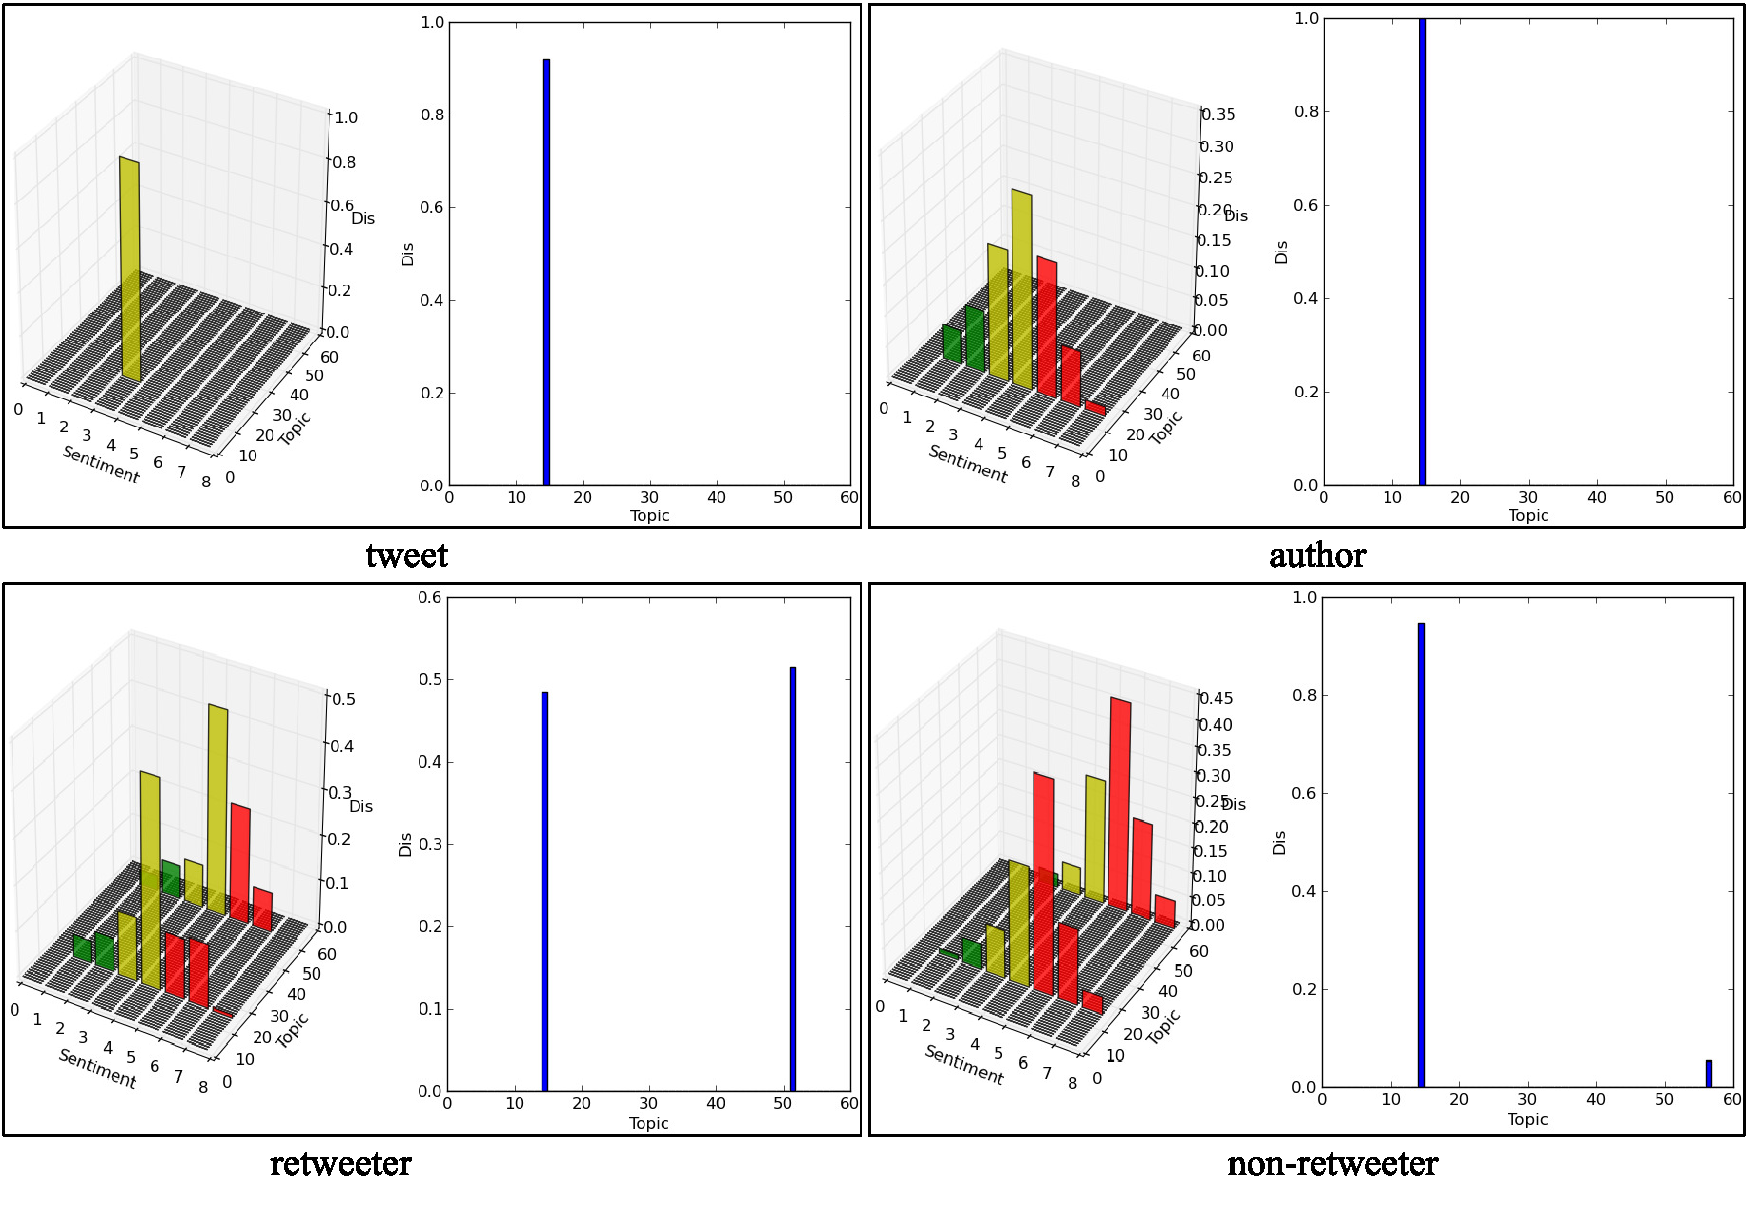
\includegraphics[height=320pt]{6-2.pdf}
\caption{主观模型示意图}
\label{fig6-2}
\end{figure}

图~\ref{fig6-3}显示了$ 14^{th} $号话题、微博作者与两个关注者的所有微博的词云图(word cloud diagrams)\footnote{我们使用TagCrowd (\url{http://tagcrowd.com/})生成词云图。}。

\begin{figure}[htb]
\centering
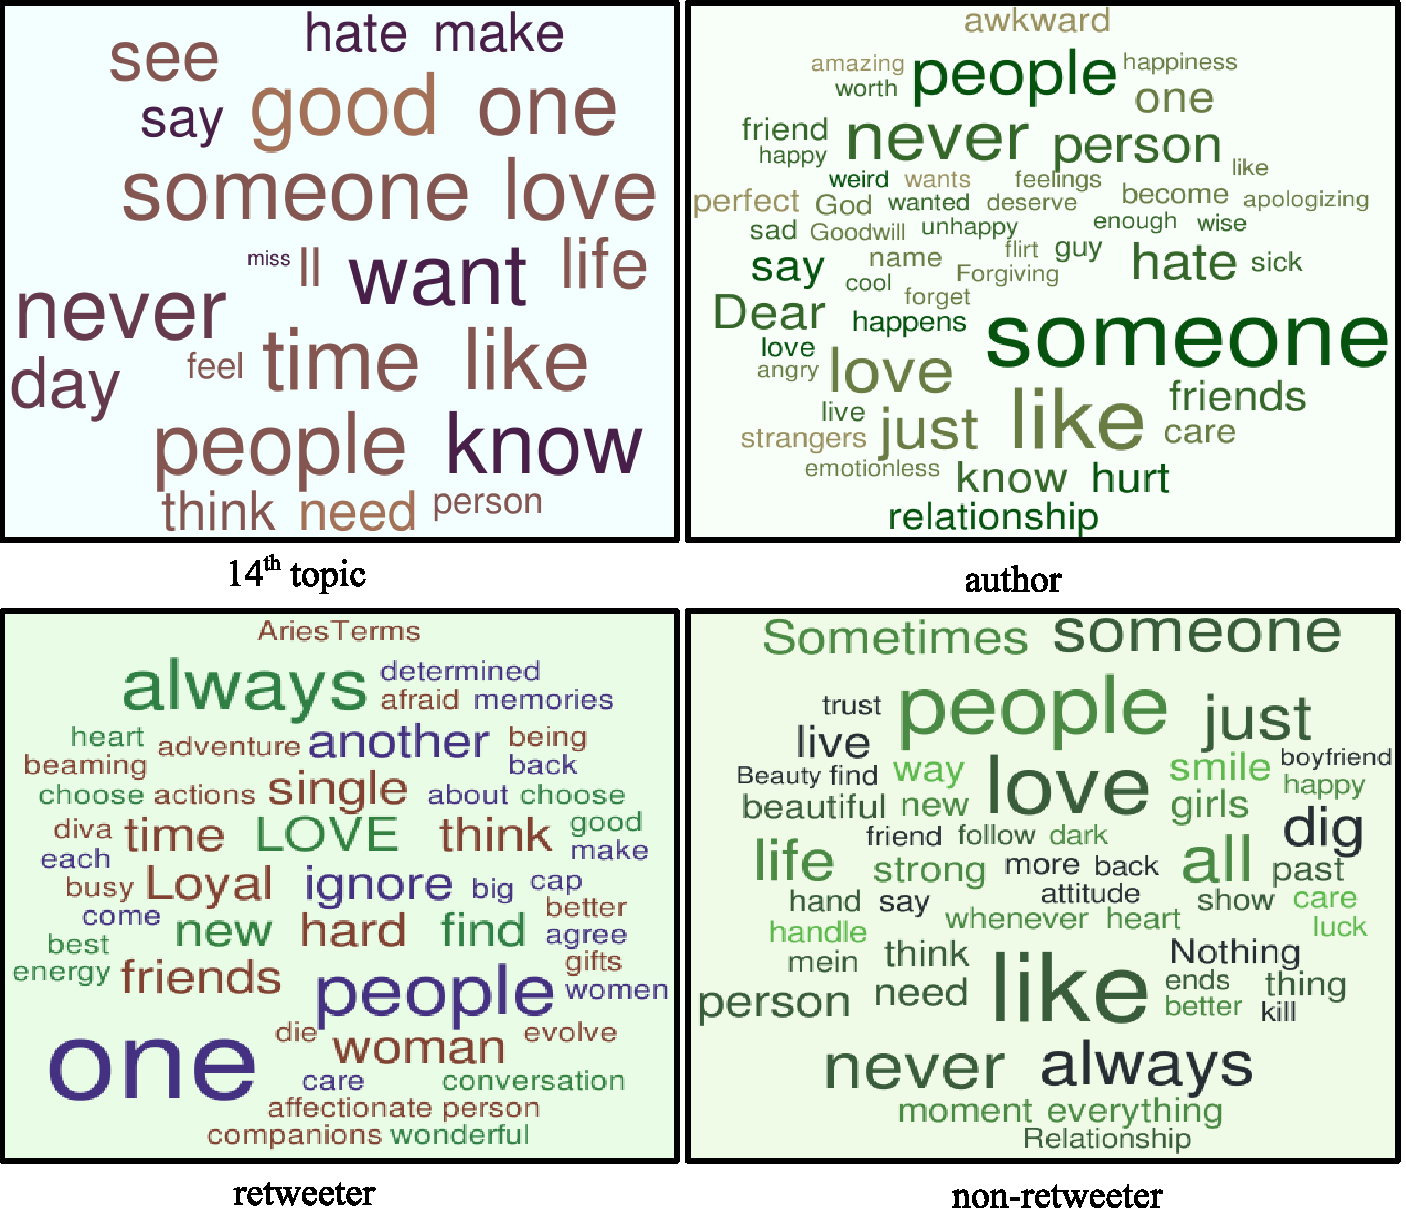
\includegraphics[height=320pt]{6-3.pdf}
\caption{$ 14^{th} $号话题、微博作者与两个关注者词云图}
\label{fig6-3}
\end{figure}

该微博谈论的是$ 14^{th} $号话题,话题是关于“love between people”,且作者对该话题的观点偏中性,可以看出这与图~\ref{fig6-2}中微博的主观模型以及图~\ref{fig6-3}中$ 14^{th} $号话题词云图是一致的;
微博作者有188条微博,主要集中在$ 14^{th} $号话题,观点分布为$O_{u_{a}}^{14} =( 0, 0.04, 0.05, 0.25, 0.35, 0.25, 0.05,  0.01 )$,偏中性;至于两个关注者,转发者有196条微博,主要涉及$ 14^{th} $号话题和$ 52^{nd} $号话题,话题分布比较均匀(其中$ w_{u_{r}}(14)=0.48 $),对$ 14^{th} $号话题,观点分布为$O_{u_{r}}^{14} =( 0, 0.02, 0.04, 0.15, 0.50, 0.13,  0.15,  0.01)$,偏中性;未转发者有156条微博,涉及到$ 14^{th} $号话题和$ 56^{th} $号话题,主要谈论了$ 14^{th} $号话题(其中$ w_{u_{n}}(14)=0.98 $),观点分布为$O_{u_{n}}^{14} =( 0, 0.01, 0.04, 0.10, 0.25, 0.45, 0.13, 0.02)$,偏正面。

表~\ref{tab6-4}是针对转发者和未转发者考虑三个引起转发因素计算的三个主观相似性,可以看出对于转发者来说,除了微博与其作者的主观相似性(度量微博流行性)外,其他两个主观相似性都明显高于未转发者。

\begin{table}[htp]
\centering
\caption{主观相似性比较}
\label{tab6-4}
\begin{tabular}{|c|c|c|c|}
\hline
相似性 & $ Sim(f,t) $ & $ Sim(f,u_a)  $ & $ Sim(u_a,t)  $\\
\hline
Retweeter & 0.854 & 0.967 & 0.886\\
\hline
Non-retweeter & 0.805 & 0.919 & 0.886\\
\hline
\end{tabular}
\end{table} 

从以上分析中看得出,对于微博的两个关注者,仅就感话题兴趣度来说,未转发者与微博以及微博作者更为相似(在共同话题$ 14^{th} $话题的兴趣度:作者$ w_{u_{a}}(14)=1.0 $,未转发者$ w_{u_{n}}(14)=0.98 $,转发者$ w_{u_{r}}(14)=0.48 $),但是考虑到主观相似性,转发者因为与微博以及作者有更相似的观点分布因而主观相似性更高(与微博主观相似性(度量吸引力)$ Sim(f,t)$:0.854 vs 0.805,与作者主观相似性(度量社交性)$ Sim(f,u_a)  $:0.967 vs 0.919),因此主观相似性的不同引发了他们不同的转发行为,从这个例子可以看出主观模型结合三个因素的主观相似性度量在解释用户转发行为上的作用。

\subsection{转发预测}
为了进一步定量的评价所提出的方法的有效性,分三阶段进行了转发预测实验。

首先,将本章模型与其他基于话题的模型进行对比实验。对比模型包括使用词袋模型对用户兴趣建模的TF-IDF模型、从用户产生内容中抽取实体对用户兴趣建模的基于实体模型(entity)以及使用用户微博中的hashtag的hashtag模型\upcite{Abel2011},对这些模型计算相似性的时候使用的是余弦相似性。

第二个阶段,将本章模型与两个话题情感生成模型(generative topic-sentiment models)TSM模型\upcite{Mei2007}以及JST模型\upcite{Lin2009}进行了对比实验。虽然TSM模型和JST模型也能同时对话题和话题相关的情感建模,但是他们的情感输出为正负二值极性。在训练这两个模型时,同样也是将用户所有微博作为一篇文档输入,并且使用本章定义的主观相似性计算方法~\ref{subsim}来计算三个主观相似性,但是在实际使用中是将三个相似性值组合起来作为特征同时加入到分类器中评价模型的预测性能。

第三个阶段,考虑到影响转发行为的其他因素,比如网络结构或用户Twitter使用习惯等元数据,也将本章模型和综合考虑其他因素的方法进行了对比。在此主要是和Luo\upcite{Luo2013}的工作(标记为“LUO”)进行了对比,表~\ref{tab6-5}是Luo\upcite{Luo2013}的模型使用的一些特征。
\begin{table}
\centering
\caption{LUO方法使用特征}
 \label{tab6-5}
  \begin{tabular*}{\textwidth}{@{\extracolsep{\fill}}| l l p{1.7in}|} 
 \hline 
\textbf{转发历史特征(RH)} & \textbf{取值范围} & \textbf{Description} \\
 \hline
  用户转发数目(Num\_fRu)& $N=\{0,1,2,...\}$ & 粉丝转发作者tweet的数目 \\
  用户提及数目(Num\_fMu)& $N=\{0,1,2,...\}$ & 粉丝提及作者tweet的数目 \\
  用户被转发数目(Num\_uRf)& $N=\{0,1,2,...\}$ & 作者转发粉丝tweet的数目 \\
  用户被提及数目(Num\_uMf)& $N=\{0,1,2,...\}$ & 作者提及粉丝tweet的数目 \\
  用户转发比例(Ratio\_retweet)& $[0,1]$ & 粉丝的tweet中转发tweet的比例 \\
  用户提及比例(Ratio\_mention)& $[0,1]$ & 粉丝的tweet中提及tweet的比例 \\
  \hline
 \hline
\textbf{用户特征(FS)} & \textbf{取值范围} & \textbf{Description} \\
 \hline
 发布tweet数目(Posts)  & $N^+=\{1,2,3,...\}$ & 作者以往发布tweet的数目 \\  
 粉丝数目(Followers) &$N=\{0,1,2,...\}$& 作者的粉丝数目 \\
 朋友数目(Friends)  & $N=\{0,1,2,...\}$ & 作者的朋友数目 \\
 分组数目(Listed)  &$N=\{0,1,2,...\}$& 作者的分组数目  \\
 验证用户(Verified)& $0$ or $1$ &  作者是否被官方验证\\
 \hline
 \hline
\textbf{用户活跃时间特征(FAT)} & \textbf{取值范围} & \textbf{Description} \\
 \hline
 时区时间(Timezone)& $0$ or $1$ &  粉丝是否与作者在同一个时区\\
 用户户活跃时间(PostTimeConsis)& $[0,1]$ & 粉丝发布tweet不同时间的数目比例 \\
\hline
 \hline
 \textbf{用户兴趣特征(FI)} & \textbf{取值范围} & \textbf{Description} \\
  相似兴趣(SimInterest)& $(-1,1)$ & tweet与粉丝以往发布tweet的相似度 \\
\hline
 \end{tabular*}
\end{table}
其中对用户兴趣建模部分,LUO方法使用的是简单的词袋模型,为了验证本章提出的方法在预测转发行为时的作用,实验将LUO方法中的用户兴趣特征替换为本章的三个主观相似性指标作为特征进行组合实验(使用“LUO+”前缀表示)。


实验中使用的是逻辑回归分类器(logistic regression classifier),用5倍交叉验证方式(5-fold cross-validation)训练测试,评价指标采用准确率。对于基准(baseline)设置,采用了一个基本的基准,该基准假设如果一个粉丝曾经转发目标微博作者的的微博,那么他很有可能会继续转发,因此直接将其预测为目标微博的转发者。
准确率结果如表~\ref{tab6-6}所示。

\begin{table}[htb]
\centering
\caption{准确率评测结果}
\label{tab6-6}
\begin{tabular}{|l|l|l|l|}
\hline
特征 &准确率(\%) & 特征 &准确率(\%)\\
\hline
baseline & 60.85 & & \\
\hline
TF-IDF & 62.85   $\ast$ & LUO & 71.76 $ \ast  $\\
entity & 68.76  $\ast$ & LUO+entity & 72.15 $\ast$\\
hashtag & 59.12  & LUO+hashtag & 68.44 $\ast$\\
\hline
TSM & 67.44 $\ast$ & LUO+TSM & 68.23 $\ast$\\
JST & 68.13 $\ast$ & LUO+JST & 70.53 $\ast$\\
\hline
$ Sim(f,t) $ & 73.88   $\ast  \quad \ddagger $ &LUO+$ Sim(f,t)$ & 74.04  $ \ast \quad \ddagger $\\
$ Sim(f,u_a)  $ & 70.04   $\ast  $ & LUO+$ Sim(f,u_a)$ & 70.27  $ \ast $\\
$ Sim(u_a,t)  $ & 69.64   $\ast  $ & LUO+$ Sim(u_a,t)$ & 71.86  $ \ast $\\
$ sim_{all}  $ & \textbf{75.64}   $\ast \quad \ddagger $ & LUO+$ sim_{all}  $ & \textbf{78.15}  $ \ast \quad \ddagger $\\
\hline
\end{tabular}
\begin{tablenotes}
  \centering
  \footnotesize
\item 显著性水平($p < 0.05$),使用$ \ast $标记性能显著超过基准,\\
\item 用$ \ddagger $标记性能显著超过LUO。
\end{tablenotes}
%\end{threeparttable}
\end{table}
从表中可以看出:
\begin{itemize}
\item 首先,除了hashtag模型外,其他模型的准确率都显著超过了基准准确率(60.85\%),hashtag模型准确率为59.12\%,准确率低的主要原因是微博中hashtag的使用率过低而造成的数据稀疏。
\item 第二,对比实验中,两个主观相似性指标$ Sim(f,t) $和$ sim_{all}  $准确率显著超过了LUO方法(71.76\%),其中最高准确率为$ sim_{all}  $(75.64\%),是将三个主观相似性组合起来作为特征加入到分类器中,TF-IDF模型(62.85\%)仅仅比基准准确率稍好,entity模型(68.76\%)准确性接近 $ Sim(f,u_a)$(70.04\%)和$ Sim(u_a,t)  $(69.64\%),差别并不显著。
\item 第三,两个生成模型(TSM: 67.44\%,JST: 68.13\%)准确率不如本章提出的模型,主要原因在于他们的情感表示形式是二值极性表示,不能够很好的区分不同的观点,而我们的模型采用新的在情感空间的分布表示,可以区分用户细致的观点差别,从而可以对用户转发行为的主观动机建模。
\item 最后,在组合实验中,$ Sim(f,t) $指标对准确率的提高显著(LUO+$ Sim(f,t) $,准确率提高2.12\%),但是其他两个主观相似性以及entity模型加入后准确率提高不明显,加入hashtag和两个生成模型后准确率反而会降低,值得注意的是将三个主观相似性同时加入到LUO方法中准确率提高最多(LUO+$ sim_{all}  $,准确率提高6.39\%)。
\end{itemize}

综上所述,转发预测结果显示主观模型以及考虑三个因素的主观相似性可以很好的预测用户的转发行为,能够作为分析转发行为的有效途径。

\section{小结}
本章在前面主观模型的基础上从主观动机角度对用户的转发行为的进行了分析,提出了新的主观相似性计算方法,并通过考虑影响用户转发行为的微博吸引力、朋友间的社交性以及微博的流行性三个不同因素,对用户的转发行为进行分析,并将三个因素量化为三个主观相似性。实验结果证明了主观相似性与转发行为存在相关性,可以很好的解释和预测用户的转发行为,对于理解用户的转发行为的主观动机有重要作用。

